\documentclass{article}
\usepackage{graphicx}
\usepackage{xcolor}
\usepackage[utf8]{inputenc}
\usepackage[T1]{fontenc}
\renewcommand{\rmdefault}{ptm}
\renewcommand{\sfdefault}{ptm}
\renewcommand{\ttdefault}{ptm}
\usepackage[french]{babel}
\usepackage{textcomp}
% Si vous voulez réinitialiser la numérotation des sections et pages à un certain point
\usepackage{titlesec}
\usepackage{url}
\usepackage{ragged2e}
\usepackage{enumitem}
\usepackage[a4paper, margin=2.5cm]{geometry}  % Ajuster les marges à 2.5 cm de chaque côté
\renewcommand{\thesection}{\arabic{section}} % Utiliser des chiffres arabes pour la numérotation des sections

\begin{document}
% Page de couverture
\begin{titlepage}
    \centering
    
\includegraphics[width=0.4\textwidth]{resourse/logoSorbonne.png}
    \begin{center}
        \hrulefill \\[1cm]
        \Huge\textbf{Sorbonne Université} \\[1cm]
        \Large\textbf{Master 2 Science et Technologie du Logiciel} \\ [1cm]
        \hrulefill \\[2cm]
        \huge\textbf{Rapport du projet1 DAAR : Automate } \\[1cm]
        \huge\textbf{\textcolor{cyan}{Clone de egrep avec support partiel des ERE}} \\[2cm]
        \hrulefill \\[2.5cm]
        \Large\textbf{Auteur:} Nandraina RAZAFINDRAIBE\\[0.5cm]
        \Large\textbf{Auteur:} Florian CODEBECQ\\[0.5cm]
        \Large\textbf{Responsable:} Binh-Minh BUI-XUAN\\[2.5cm]
        \textbf{Année scolaire:} 2024/2025  
    \end{center}
\end{titlepage}

% Page suivant %
\newpage
\setcounter{page}{1}

\setcounter{section}{0}
\section{Introduction}
Dans ce projet, nous avons développé un clone partiel de la commande Linux egrep, capable de rechercher des motifs dans un fichier textuel à l'aide d'expressions régulières étendues (ERE). L'objectif principal est d'explorer plusieurs approches d'implémentation des algorithmes de recherche de motifs, et d'analyser leurs performances.

Pour la réalisation du projet, nous avons décidé d'utiliser Java comme langage de programmation.

\section{Problématique et Objectifs}
Le problème à résoudre est la recherche de motifs dans des fichiers textuels en utilisant des expressions régulières conformes à la norme ERE. Deux stratégies principales sont considérées :

\begin{itemize}
    \item Automates : Transformation de l'expression régulière en automate fini non déterministe (AFND) avec $\epsilon$-transitions, puis en automate fini déterministe (AFD) via la méthode des sous-ensembles.
    \item Recherche linéaire : Utilisation de l'algorithme Knuth-Morris-Pratt (KMP) pour la recherche de motifs simples.
\end{itemize}

\section{Méthodologie}
\subsection{Méthode d’Aho-Ullman}
Cette approche consiste à construire un automate fini à partir d’une expression régulière. Pour parvenir à notre objectif, on doit passer sur plusieurs étapes:
\begin{itemize}
    \item Construction d'un arbre syntaxique à partir d’\textbf{une expression régulière}.
    \item Conversion de cet arbre en \textbf{un automate fini non déterministe (AFND)} avec $\epsilon$-transition.
    \item Transformer de l’automate fini non déterministe en \textbf{un automate fini déterministe (AFD)}.
    \item Optimiser l’AFD afin d’obtenir un automate avec un nombre minimum d’états.
    \item Rechercher les motifs avec l’automate ainsi obtenu.
\end{itemize}

\subsubsection{Une expression régulière vers l’arbre syntaxique}
Cette étape réalise une analyse syntaxique du motif entré par l'utilisateur en identifiant les opérations à effectuer sur les caractères qui le composent. Les opérations respectent l'ordre de priorité suivant : les parenthèses "()", les quantificateurs "*", la concaténation ".", et l'alternance "|".

Pour ce projet, un code en Java a été fourni dès le départ, qui prend en entrée une expression régulière et retourne l'arbre syntaxique correspondant. Nous avons ensuite basé la suite du projet sur ce code.
\subsubsection{Construire l’automate fini non déterministe}
Nous devons définir des règles pour chaque opération dans l'arbre syntaxique afin de les combiner et, en fin de compte, générer l'automate correspondant. Pour clarifier ce processus, prenons l'exemple de l'arbre " .(a,b)".

Ci-dessous, nous montrons l'équivalence entre sa représentation en graphe et son équivalent sous forme de tableau. Lors de la transformation en automate, chaque lettre est représentée par un minimum de 4 états.

\begin{figure}[h]
    \begin{minipage}{0.3\textwidth}
        \centering
        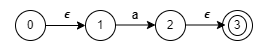
\includegraphics[width=\textwidth]{resourse/NDFA_a.png}
        \caption{Automate fini non déterministe de "a"}
        \label{fig:ndfa_a}
        \cite{ndfa_a}
    \end{minipage}
    \hspace{5cm} % Espace horizontal entre les deux images
    \begin{minipage}{0.25\textwidth}
        \centering
        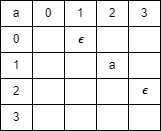
\includegraphics[width=\textwidth]{resourse/NDFA_a.tab.png}
        \caption{Représentation sous forme de tableau de "a"}
        \label{fig:ndfa_tab_a}
        \cite{ndfa_tab_a}
    \end{minipage}
\end{figure}

\newpage
\begin{figure}[h]
    \begin{minipage}{0.3\textwidth}
        \centering
        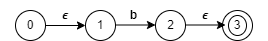
\includegraphics[width=\textwidth]{resourse/NDFA_b.png}
        \caption{Automate fini non déterministe de "b"}
        \label{fig:ndfa_b}
        \cite{ndfa_b}
    \end{minipage}
    \hspace{5cm} % Espace horizontal entre les deux images
    \begin{minipage}{0.25\textwidth}
        \centering
        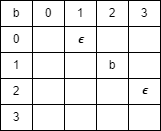
\includegraphics[width=\textwidth]{resourse/NDFA_b.tab.png}
        \caption{Représentation sous forme de tableau de "b"}
        \label{fig:ndfa_tab_b}
        \cite{ndfa_tab_b}
    \end{minipage}
\end{figure}

Cette étape consiste à remonter dans l'arbre tout en combinant les feuilles, en commençant par le niveau le plus profond. Les opérations indiquées sur les nœuds dictent les règles à suivre pour effectuer la combinaison.

\begin{figure}[h] % Utilisation de l'option [h] pour placer l'image ici
    \centering
    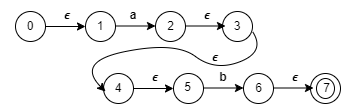
\includegraphics[width=0.45\textwidth]{./resourse/NDFA_ab.png}
    \caption{Automate fini non déterministe de l'arbre ".(a,b)"}
    \cite{ndfa_ab}
    \label{fig:ndfa_ab}
\end{figure}

Pour la règle de concaténation ".", nous avons ajouté une nouvelle transition $\epsilon$ entre l'état 3 (ancien état d'acceptation de l'AFND gauche) et l'état 4 (état de départ de l'AFND droit).

Le tableau suivant correspond à l'AFND du graphe \cite{ndfa_ab} :
\begin{figure}[h] % Utilisation de l'option [h] pour placer l'image ici
    \centering
    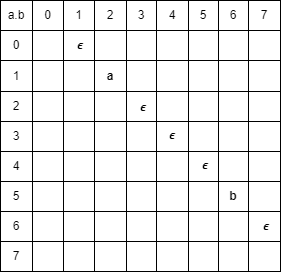
\includegraphics[width=0.38\textwidth]{./resourse/NDFA_ab.tab.png}
    \caption{Représentation sous forme de tableau de l'arbre ".(a,b)"}
    \cite{ndfa_tab_ab}
    \label{fig:ndfa__tab_ab}
\end{figure}

Pour les autres opérations, telles que l'étoile "*" et l'alternance "|", l'idée reste similaire, mais les règles diffèrent légèrement. Ces règles sont définies dans des méthodes d'une classe. Des appels de ces méthodes sont ensuite effectués jusqu'à atteindre la racine de l'arbre, afin de générer \textbf{un tableau à deux dimensions de caractères} représentant les transitions de l’automate .

\subsubsection{Convertir l’automate fini non déterministe en déterministe}
À partir de l'AFND, nous cherchons à éliminer toutes les transitions $\epsilon$ intermédiaires pour rendre l'automate déterministe en utilisant la méthode des sous-ensembles. Cette méthode commence par définir l'état de départ de l'AFD, qui est lui-même un ensemble d'états de l'AFND. Les états de l'AFD sont stockés dans des structures de type \textbf{HashSet} afin de garantir leur \textbf{unicité}.

En parcourant les sous-ensembles de tous les états de l'AFD, nous cherchons à déterminer si une transition existe pour chaque caractère d'entrée possible dans l'AFND.

Si c'est le cas, nous continuons le parcours tant que les transitions vers les autres états successeurs sont des transitions $\epsilon$. Ensuite, nous ajoutons les sous-ensembles des états successeurs comme nouveaux états de l'AFD. Le parcours s'arrête lorsqu'il n'y a plus d'états dans l'AFD nécessitant d'être parcourus.

Si l'un des sous-ensembles d'états de l'AFD contient l'état initial de l'AFND, cet état de l'AFD est défini comme état initial. De même, si un sous-ensemble contient l'état d'acceptation de l'AFND, cet état de l'AFD est défini comme état d'acceptation.

La structure de données utilisée pour stocker l'AFD est le \textbf{HashMap<String, HashMap<String, String>}. Les états de départ et d'acceptation sont stockés avec un \textbf{HashMap<String, Boolean>}. Ces choix de structures de données visent à optimiser l'allocation mémoire tout en permettant également une récupération rapide des états et des transitions grâce à son accès en temps constant O(1).

\subsubsection{Réduction de l'AFD (Minimisation)}
L'optimisation la plus courante pour un AFD est la \textbf{minimisation}. Réduire le nombre d'états tout en conservant les mêmes propriétés de reconnaissance du langage. Dans ce projet, on a utilisé un algorithme de partitionnement des états souvent appelé algorithme de Moore.

La première étape consiste à identifier les états atteignables à partir de l'état initial. Cette opération est réalisée en utilisant une exploration en largeur (BFS). Tous les états qui ne peuvent être atteints sont supprimés de l'automate, ce qui simplifie l'AFD en éliminant des états inutiles, rendant ainsi le calcul plus efficace, plus rapide et optimise l’utilisation de la mémoire. 

Dans le processus de partitionnement des états équivalents, on commence par diviser les états en deux groupes principaux : les \textbf{états finaux} et les \textbf{états non-finaux}, qui ne peuvent jamais être équivalents.

Par la suite, chaque groupe est progressivement subdivisé en fonction des transitions. Deux états sont dits équivalents s'ils ont les mêmes transitions vers des groupes identiques d'états. Pour cela, une méthode de signature est utilisée, où chaque état est caractérisé par la "signature" des états vers lesquels il se dirige. Si deux états partagent la même signature, ils sont considérés comme équivalents.

Cette étape se répète jusqu'à ce que les partitions ne puissent plus être subdivisées, assurant ainsi que chaque groupe contient des états totalement équivalents. Une fois les partitions stables identifiées, les états équivalents sont fusionnés. Cela se traduit par la création d’un mapping qui associe chaque ancien état à un état représentant l'ensemble des états équivalents. Cette fusion réduit le nombre total d’états dans l’automate tout en gardant son comportement.

À la fin du processus, un nouvel automate est construit en appliquant le mapping des états équivalents, créant ainsi un \textbf{AFD minimisé} qui contient moins d'états mais accepte le même langage que l’automate original.

\subsubsection{Recherche de motif}
Les étapes de recherche des motifs dans un fichier .txt donnée peuvent être réparties en 3 étapes:

\begin{itemize}
    \item Une méthode qui  prend une ligne de texte à partir d'une position donnée et vérifie si une sous-chaîne est acceptée par l'AFD .Le parcours commence à l’état initial et se déplace selon les transitions de l’automate, vérifiant chaque symbole. Si un état final est atteint, la sous-chaîne est acceptée.
    \item La méthode qui vérifie dans une ligne parcourt chaque sous-chaîne possible d’une ligne pour trouver des correspondances avec l’automate. Si une sous-chaîne est acceptée, la ligne est validée.
    \item On parcourt chaque ligne d’un fichier et applique la vérification. Les lignes contenant des sous-chaînes acceptées sont affichées avec leur numéro.
\end{itemize}

\subsection{Algorithme Knuth-Morris-Pratt (KMP)}
L'algorithme de Knuth-Morris-Pratt (KMP) est un algorithme de recherche de sous-chaîne dans une chaîne de caractères.

Cet algorithme utilise une technique de prétraitement pour créer un tableau d'indices de décalage (LPS - Longest Prefix Suffix), ce qui permet de sauter des comparaisons inutiles et d'optimiser la recherche. Il est basé sur l'idée de ne pas comparer les caractères qui ont déjà été comparés. Au lieu de cela, il utilise un tableau d'indices de décalage pour sauter les comparaisons inutiles.

Voici la méthodologie du déroulement de l’algorithme KMP :

\begin{itemize}
    \item Prétraitement du motif : Calculer le tableau LPS du motif. Ce tableau aide à déterminer jusqu'où le motif peut être décalé en cas de désaccord partiel lors de la recherche dans le texte.
    \item Recherche dans le texte : Parcourir le texte de manière linéaire tout en exploitant le tableau LPS pour éviter de revérifier les caractères qui correspondent déjà.
\end{itemize}

\section{Test et Analyse de performance}

\newpage
\bibliographystyle{unsrt}
\bibliography{references}
\end{document}